% !TEX root = ../thesis_main.tex
%
%
%
%%%% --- * --- %%%%	
\clearpage
\chapter{The Experimental Setup}
%\label{atomicphysics_chapter}
\label{experimental_chapter}
\section{An Overview of the Double MOT System and Duty Cycle}
\label{section:overview}
\label{setup_chapter}
\note{put this in!  ``....and is designed to operate at ultra-high vacuum (UHV) to minimize trap losses from collisions.''  Also, I think it helps prevent sparking?}
%
\note{Remember the pulser LED!  To evaluate the stability of the scintillator gain!}


The experimental subject matter of this thesis was conducted at TRIUMF using the apparatus of the TRIUMF Neutral Atom Trap (TRINAT) collaboration.  The TRINAT laboratory offers an experimental set-up which is uniquely suited to precision tests of Standard Model beta decay physics, by virtue of its ability to produce highly localized samples of cold, isotopically pure atoms within an open detector geometry.  \aside[org]{Surely most of this paragraph goes in an intro chapter somewhere.}  Although the discussion in this chapter will focus on the methodologies used to collect one particular dataset, taken over approximately 7 days of beamtime in June 2014, the full apparatus and the techniques used are fairly versatile, and can be (and have been) applied to
several related experiments using other isotopes.
\note{Cite a bunch of papers here.}

\begin{figure}[t!h]
	\centering
	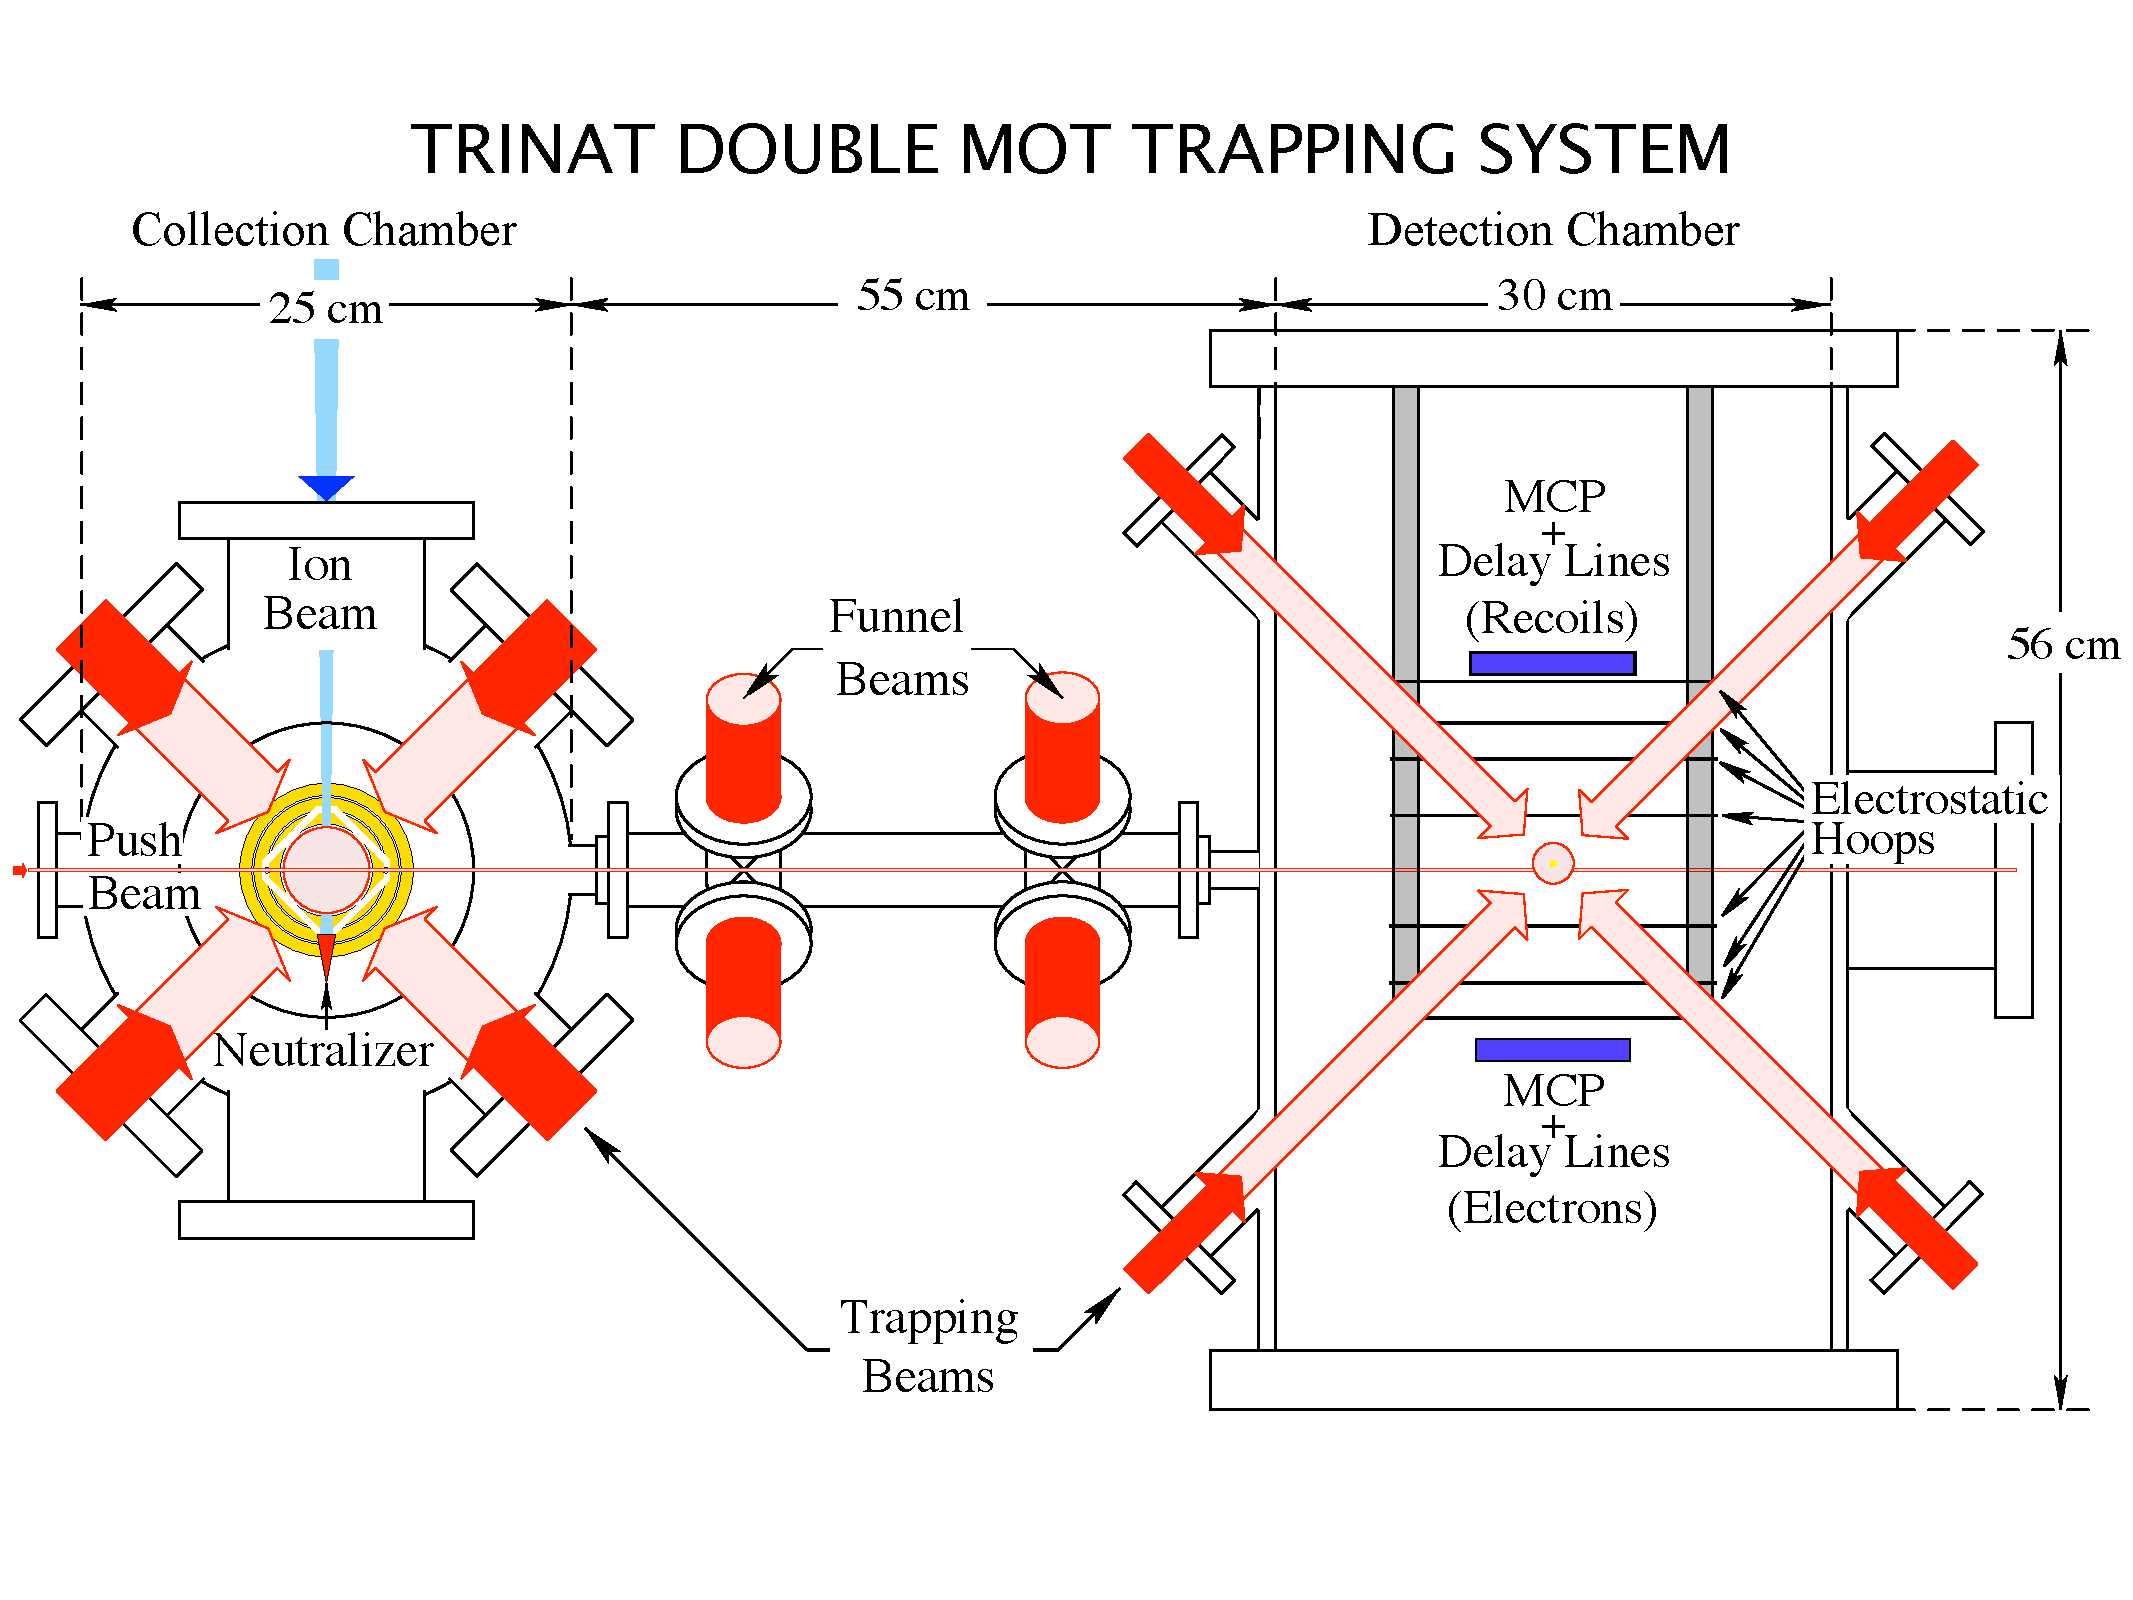
\includegraphics[width=.999\linewidth]
	{Figures/DoubleMot5.pdf}
	\caption[The TRINAT experimental set-up, viewed from above]{The TRINAT experimental set-up, viewed from above.  Ions from the beamline pass through the collection chamber onto the neutralizer, which is held at ground.  The neutralizer is heated to release the neutral atoms from its surface back into the collection chamber, where some are collected into a \ac{MOT}.  Atoms from the collection chamber's MOT are transferred directly into the detection chamber's MOT approximately once per second, kept focused during the transfer by funnel beams (lasers).  Within the detection chamber, background events are dramatically reduced.  }
	\label{fig:doublemot}
\note{Figure was originally created by Alexandre, modified by ... someone else?  Or Alexandre?  And I got it from ... probably an experimental proposal?  I should figure out how to cite a proposal...}
%%\note[jbnn]{In Fig 2.2 caption ``Every 16 sec the atoms are transferred''
%%\\...\\
%%no, that's every 0.71 sec, of course, or we would lose atoms by $2^{16}$ or so decaying in the first trap before tranfer, hmm?
%%(The 16 sec business is just 16 steps of a scanning parameter for tuneup-- it's arbitrary in the rest of the run.)
%%\\
%%I must be misreading this typo?
%%}
\end{figure}

The TRINAT lab accepts radioactive ions delivered by the ISAC beamline at TRIUMF.  These ions are collected on the surface of a hot zirconium foil where they are electrically neutralized, and subsequently escape from the foil into the first of two experimental chambers (the ``collection chamber").  Further details on the neutralization process are presented in a previous publication~\cite{gorelov2000}.  Within the collection chamber, atoms of one specific isotope -- for the purposes of this thesis,  \isotope[37]{K} -- are continuously collected into a magneto-optical trap from the tail end of the thermal distribution.~\aside{made possible by UHV!}  Although this procedure preferrentially traps only the slowest atoms, once trapped, atoms will be cooled further as a side-effect of the MOT's trapping mechanism.  The result is a small ($\sim\!1\,$mm diameter), cold ($\sim\!1\,$mK) cloud of atoms of a particular isotope.  

These properties of the atomic cloud allow for a relatively clean transfer of linear momentum from an appropriately tuned laser beam to the atoms within the cloud, and we use this mechanism to ``push'' the atoms out of the collection MOT and into the ``detection chamber'', where they are loaded into a second MOT (see Fig.~\ref{fig:doublemot}).  During regular operation, atoms are transferred approximately once per second.  

There is no need to release previously trapped atoms in the second MOT when a new group of atoms is loaded.  Although the trap loses atoms over time as a result of a variety of physical processes,\aside{discussed ... idk, somewhere else.} during typical operation the majority of atoms loaded in a given transfer will still be trapped at the time the next set of atoms is loaded, and after several transfer cycles, something like a steady state is obtained.

Because the transfer and trapping mechanisms rely on tuning laser frequencies to specific atomic resonances, these mechanisms act on only a single isotope, and all others remain unaffected.  The result is a significant reduction of background contaminants within the detection chamber relative to initial beamline output.  The transfer methodology is discussed in some detail within the collaboration's Ref.~\cite{swanson}.

\note[jm]{Here's where Juliette is annoyed that I don't describe the Swanson method.  
\\
``On page 30 the transfer and transport description is not even summarized''
}
\note[jbnn]{After your reference to Tom Swanson's paper:
\\...\\
`Some features are critical to this experiment.
The 2nd magneto-optical ``funnel'' in Figure 2.2 was added after Ref. 90, (I assume John means Ref.~\cite{swanson} here...)
to allow extra $\gamma$-ray shielding (not shown, between the 2 funnels) of untrapped atoms on the walls of the first trap. This is important because the trapping efficiency is about 1/1000.  After the 30 msec laser pulse is on to transfer atoms, a conservative 120 msec is allowed to make sure all the transferred atoms arrive and are collected and cooled before proceeding. Although there is no data collection during that 150 msec, the 2 mm diameter push laser beam is aligned several millimeters high with respect to the 2nd trap cloud to make sure all undecayed atoms are kept.'
}

We now turn our attention to what happens to the atom cloud in the detection chamber between loading phases (see Fig.~\ref{fig:dutycycle}).  One of the goals for the 2014 $^{37}\textrm{K}$ beamtime required that the atom cloud must be spin-polarized, as well as being cold and spatially confined.  Although the MOT makes it straightforward to produce a cold and well confined cloud of atoms, it is fundamentally incompatible with techniques to polarize these atoms. The physical reasons behind this are discussed in Section~\ref{section:acmot_and_polarization}.~\aside[org]{I *do* discuss this, right?  Right??}

\begin{figure}[h!!]
	\centering
	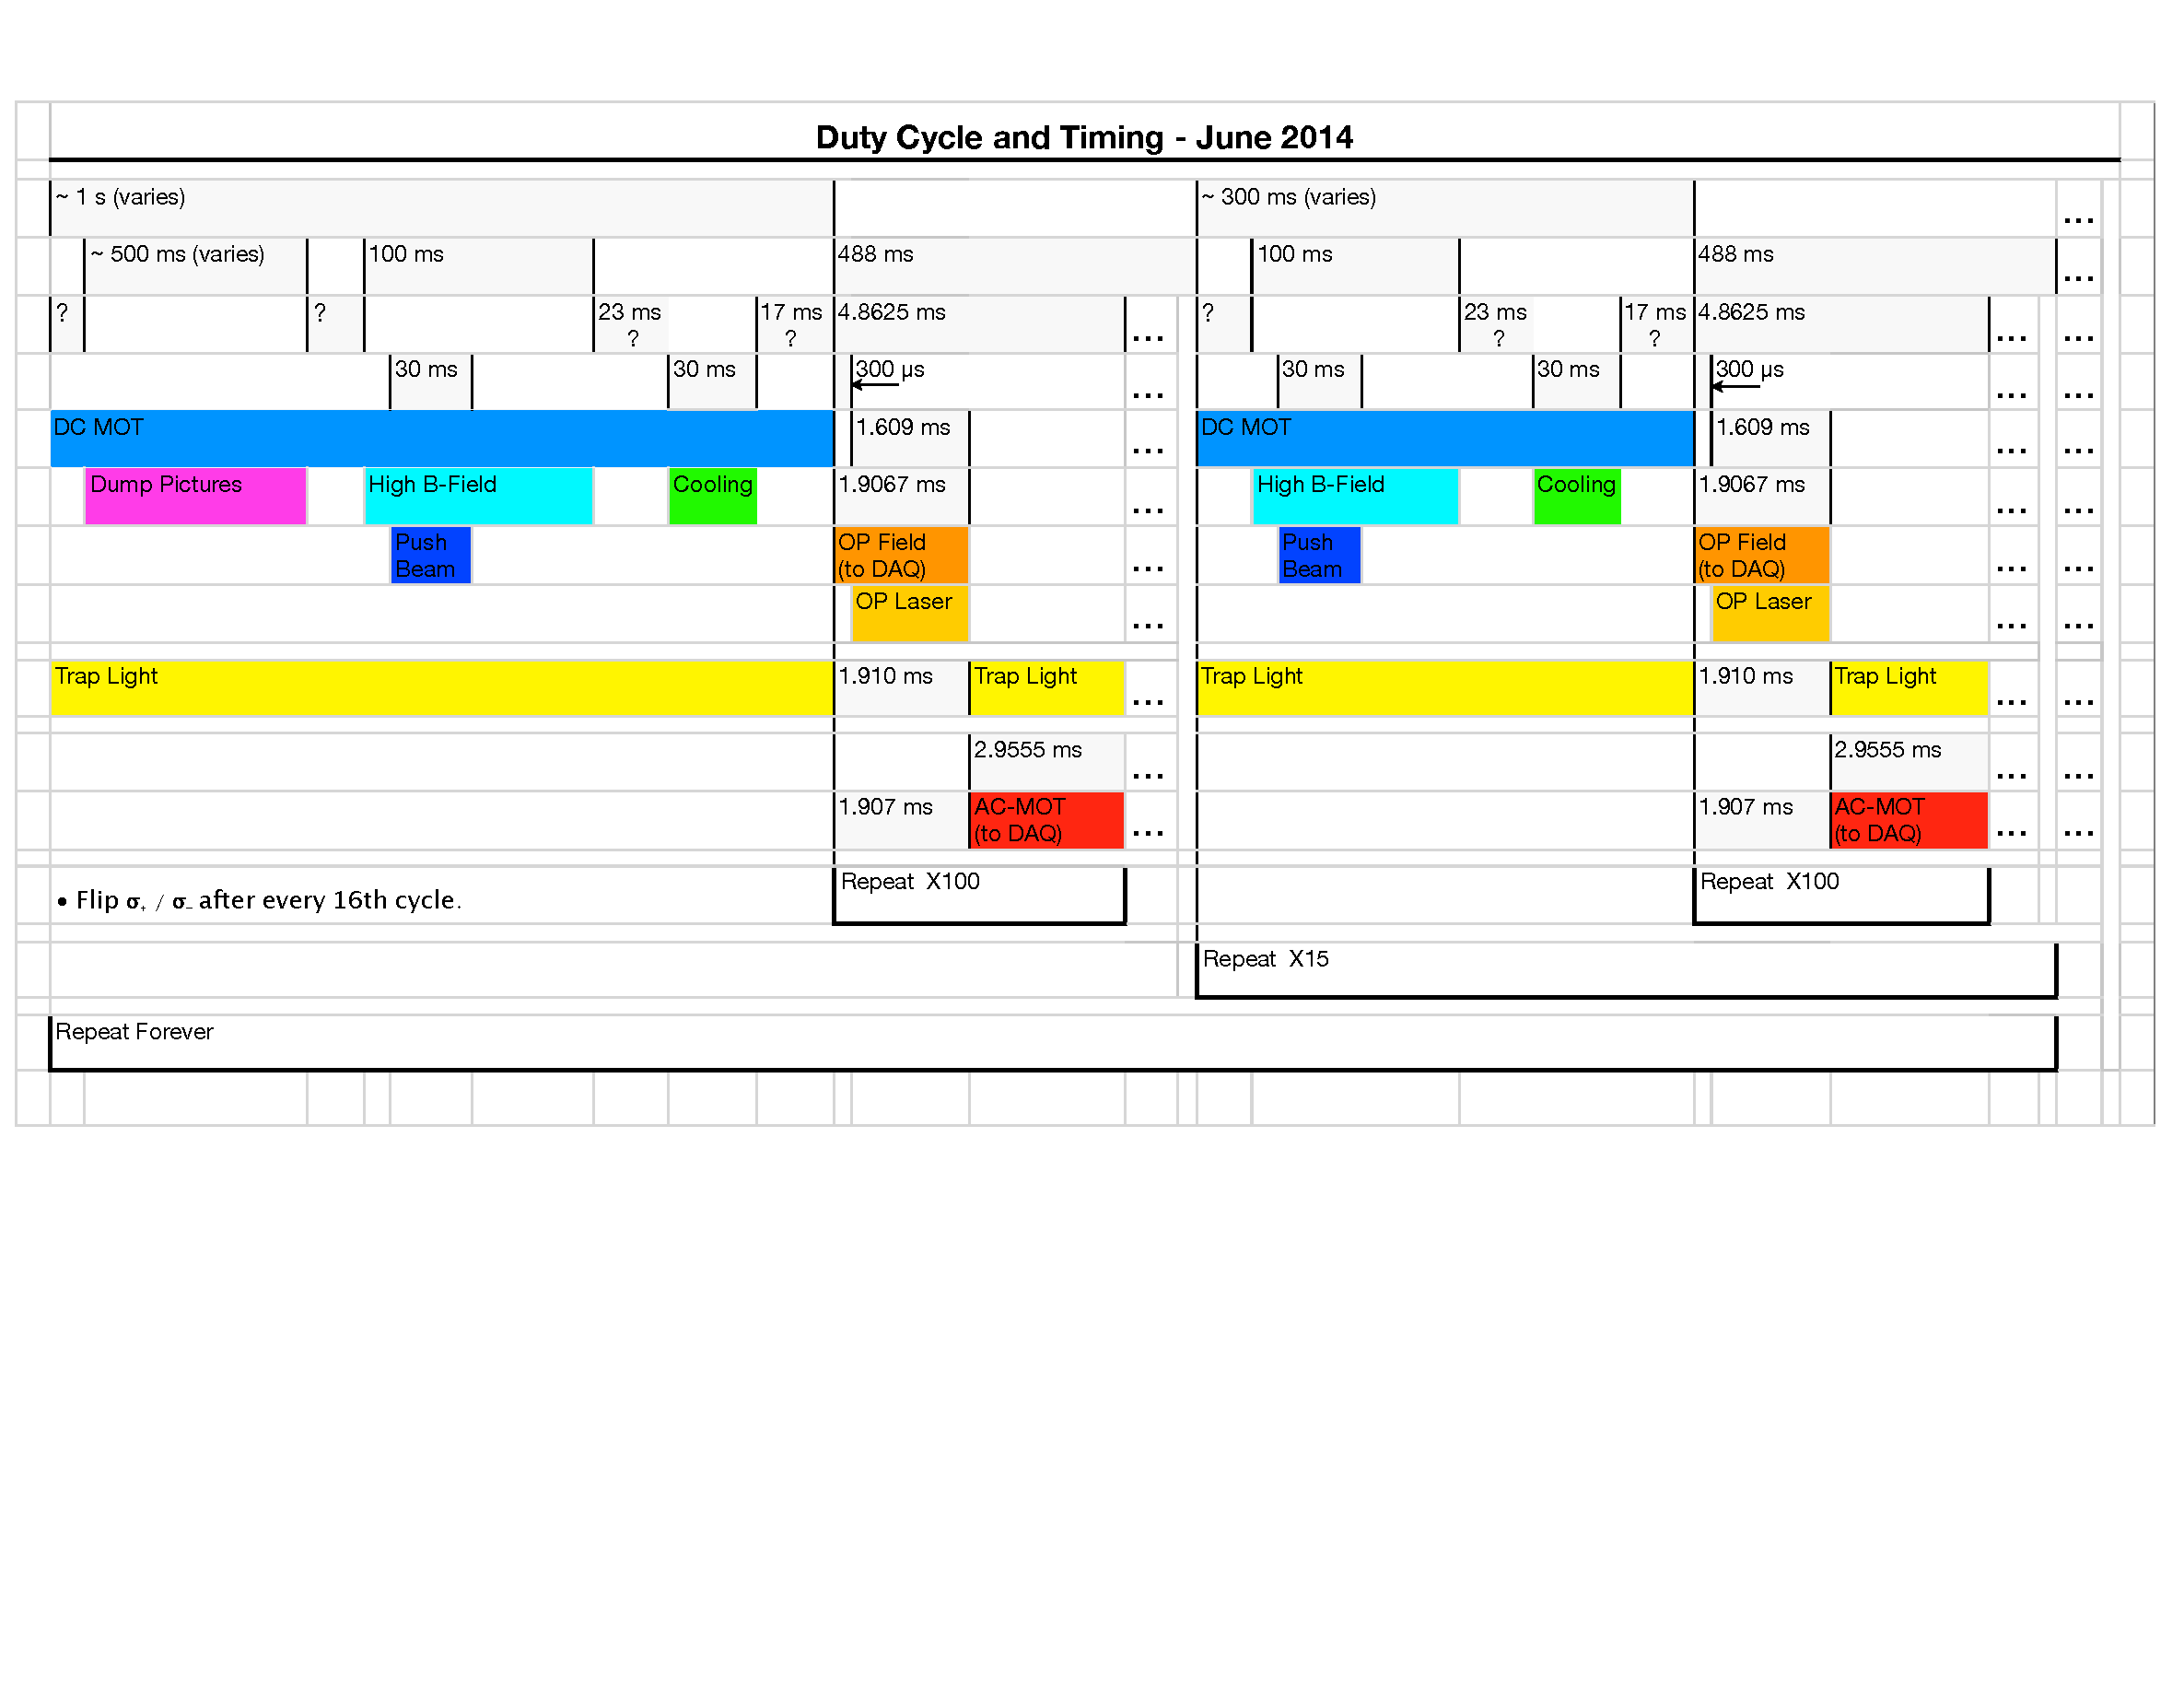
\includegraphics[width=.999\linewidth]
	{Figures/DutyCycle_2014.pdf}
	\caption[The 2014 duty cycle for transferring, cooling, trapping, and optically pumping $^{37}\textrm{K}$]{The duty cycle used for transferring, cooling, trapping, and optically pumping $\isotope[37]{K}$ during the June 2014 experiment.  Not drawn to scale.  Question marks indicate timings that varied either as a result of electronic jitter or as a result of variable times to execute the control code.  Atoms are transferred during operation of the DC-MOT.  Though the push beam laser itself is only on for $30\,$ms, the bulk of the DC-MOT's operation time afterwards is needed to collect and cool the transferred atoms.  After 100 on/off cycles of optical pumping and the AC-MOT, the DC-MOT resumes and the next group of atoms is transferred in.  After 16 atom transfers, the polarization of the optical pumping laser is flipped to spin-polarize the atoms in the opposite direction, in order to minimize systematic errors.}	
	\label{fig:dutycycle}
	\note[jbnn]{You could similarly (relative to the thing with the Swanson transfer method) comment a paragraph of critical things concerning the polarization, using your figure of the duty cycle as a guide.
	\\...\\
	``The need for highly circularly polarized light needed the highly
reflective mirrors on SiC substrates. The optical pumping process,
a biased random walk of resonant absorption of circularly polarized light,
takes about 200 microsec and limits the part of the duty cycle available for trapping, which was chosen conservatively to ensure polarization was maximized.  The nearly uniform trapping field of 2 Gauss during polarization
makes negligible perturbation of the momentum direction of the betas.
The polarization knowledge at 1/1000 accuracy removes it as a systematic for $\bFierz$ (see final table... or `it was thus left off the final table', whichever is true).
\\...\\
It is thought the largest reason for 99.1\% polarization's deviation from unity
is remaining transverse magnetic fields not along the optical pumping axis-- many details of this are in ~\cite{thesis}.'
	}
\end{figure}

Once the newly transferred set of $^{37}\textrm{K}$ atoms has been collected into the cloud, the entire MOT apparatus cycles 100 times between a state where it is `on' and actively confining atoms, and a state where it is `off' and instead the atoms are spin-polarized by optical pumping while the atom cloud expands ballistically before being re-trapped.  These 100 on/off cycles take a combined total of $488\,$ms.  The laser components of the trap are straightforward to cycle on and off on these timescales, but the magnetic field is much more challenging to cycle in this manner.  

Immediately following each set of 100 optical pumping cycles, another set of atoms is transferred in from the collection chamber to the detection chamber, joining the atoms that remain in the trap (see Fig.~\ref{fig:dutycycle}).  The details of the trapping and optical pumping cycles are described further in Section~\ref{section:acmot_and_polarization}, and the optical pumping technique and its results for this beamtime are the subject of a recent publication~\cite{ben_OP}.


\section{The Atom Transfer Methodology}
\label{sec:swansonmethod}
\note[tag]{Swanson Transfer Method}
\note[note]{Content goes here.  It probably doesn't need to be literally its own section, but still.  Content.}
%\note{}

%%% % % % %%%
\section{The AC-MOT and Polarization Setup}
%\label{sec:acmot}
\label{section:acmot_and_polarization}
\note[tag]{This section has (at one point) been literally duplicated in Chapter~\ref{sec:acmot}. When I'm done, most of the content will live *here*.}

%\note{Fix the phrasing of AC-MOT/OP experimental section.  It's passable, but still kind-of a mess.}

%The AC-MOT was first described by Harvey and Murray~\cite{harveymurray}, but the TRINAT collaboration has adopted its use because it enables the polarization-destroying magnetic field to be eliminated quickly after the MOT is shut off.  

The TRINAT collaboration has adopted the use of an AC-MOT in its detection chamber as a result of the necessity to intermittently polarize the atom cloud.  Despite the added complication, the AC-MOT is able to rapidly eliminate polarization-destroying non-uniformities in the magnetic field.  
%
Some details of the present implementation of the AC-MOT are given in Ref.~\cite{thesis}, done with a separate MOT geometry from this beta decay work.  A diagram of showing the operation phases of several key components in our AC-MOT/optical pumping duty cycle is shown in Fig.~\ref{fig:acmot}.

\begin{figure}[ht]
	\centering
		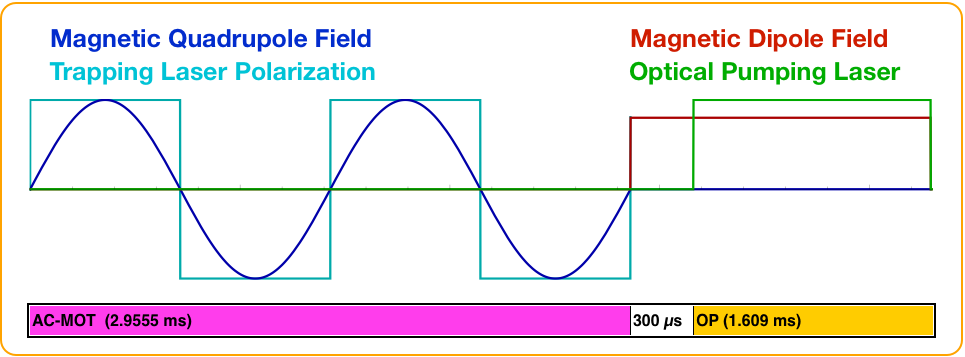
\includegraphics[width=.999\linewidth]{acmot.png}
		\caption[The AC-MOT and Optical Pumping Cycle]{One cycle of trapping with the AC-MOT, followed by optical pumping to spin-polarize the atoms.  After atoms are transferred into the science chamber, this cycle is repeated 100 times before the next transfer.  The magnetic dipole field is created by running parallel (rather than anti-parallel as is needed for the MOT) currents through the two coils.}
		\label{fig:acmot}
\end{figure}


\note[note]{}
\note[note]{Above, everything is re-edited for its current thesis location.  
\\
Below, shit's still basically duplicated in that other section.}

%A standard DC-MOT operates continuously, and in the presence of electrically conductive materials especially, the magnetic field can take a (comparatively) long time to dissipate.  This is problematic for an experiment such as this one, because the atoms do not remain confined while the magnetic field dissipates due to potential anomalies in the magnetic field shape arising from induced eddy currents, and for similar reasons, they cannot be successfully optically pumped during this time period either.  Therefore, it is important to waste as little time as possible switching between the MOT and the  optical pumping phases in the duty cycle.  For optical pumping, a weak, dipole-shaped magnetic field is preferred, and this is not possible while the quadrupole field has not dissipated.
%
%The principle behind the AC-MOT is to simply run a sinusoidal current through one's anti-Helmholtz coils while flipping the laser polarization to remain in sync.  

%\note{Eddy currents in your nearby metal objects will still be produced, and these changing eddy currents will \emph{also} create a sinusoidally oscillating magnetic field.  If correctly timed, it is possible to eliminate the current in the anti-Helmholtz coils at the precise time when the eddy currents are also eliminated.  This process can easily reduce the size of any eddy currents still produced by around an order of magnitude or more, and these remaining eddy currents decay more rapidly as well.}

\note{
%This content *came from* that other section, and needs to go in here somewhere:  
``Many laser ports to make the MOT functional, and for optical pumping.  Fancy mirror geometry to combine optical pumping and trapping light along the vertical axis.  Water-cooled (anti-)Helmholz coils within the chamber for the AC-MOT, fast switching to produce an optical pumping field.''  }

%%\note{... Sadly, this also removes our trapping mechanism.  We could keep the optical molasses after the field is off if we wanted to, but we don't, because we wouldn't be able to optically pump the atoms then.  But at least the atoms are cold-ish (we can measure!  I think it's done indirectly in that one table, or for realsies in Ben's thesis), so we can let them just chill for a little while before we have to re-trap them.  Don't lose too much.  (How much do we lose?  Have we quantified that somewhere?  Probably.).  ...}

\note{Probably document things about the waveform and frequency used for the beamtime, since I don't think it's in my MSc.}

As alluded to in the previous section~(\ref{section:overview}), the measurements in question required a spin-polarized sample of atoms, and a precise knowledge of what that polarization was.  This is needed in order to make best use of the superratio asymmetry for both $\Abeta$ and $\bFierz$ measurements.~\cite{ben_Abeta}\cite{ben_OP}.

A MOT requires a quadrupolar magnetic field, and we generate ours with two current-carrying anti-Helmholtz coils located within the vacuum chamber itself.  Since these coils are expected to run an alternating current, heat is produced and cannot be dissipated in the vacuum.  Therefore the coils themselves are hollow copper tubes, and they are continuously cooled by pumping temperature-controlled water through them.   


\note{Note that because the atoms within a MOT can be treated as following a thermal distribution, some fraction of the fastest atoms continuously escape from the trap's potential well.  Even with the most carefully-tuned apparatus, the AC-MOT cannot quite match a similar standard MOT in terms of retaining atoms.  The TRINAT AC-MOT has a `trapping half-life' of around 6 seconds, and although that may not be particularly impressive by the standards of other MOTs, it is more than adequate for our purposes.  $^{37}\textrm{K}$ itself has a radioactive half-life of only 1.6 seconds 
(cite someone), so our dominant loss mechanism is radioactive decay rather than thermal escape. }


We spin-polarize $^{37}\textrm{K}$ atoms within the trapping region by optical pumping~\cite{ben_OP}.  A circularly polarized laser is tuned to match the relevant atomic resonances, and is directed through the trapping region along the vertical axis in both directions.  When a photon is absorbed by an atom, the atom transitions to an excited state and its total angular momentum (electron spin + orbital + nuclear spin) along the vertical axis is incremented by one unit.  When the atom is de-excited a photon is emitted isotropically, 
so it follows that if there are available states of higher and lower angular momentum, the \emph{average} change in the angular momentum projection is zero.  If the atom is not yet spin-polarized, it can absorb and re-emit another photon, following a biased random walk towards complete polarization.  

In order to optimally polarize a sample of atoms by this method, it is necessary to have precise control over the magnetic field.  This is because absent other forces, a spin will undergo Larmor precession about the magnetic field lines.  In particular, the magnetic field must be aligned along the polarization axis (otherwise the tendency will be to actually depolarize the atoms), and it must be uniform in both magnitude and direction over the region of interest to avoid introducing a spatially-dependent depolarization mechanism.  
Note that this type of magnetic field is not compatible with the MOT, which requires a uniform magnetic field \emph{gradient} in all directions (characteristic of a quadrupolar field shape), and has necessitated our use of the AC-MOT.

In the end, the average (over both directions) polarization $|\vec{P}|$ achieved during the 2014 beam time is $|\vec{P}| = 0.9913 \pm 0.0009$, and the measurements are consistent with both polarization directions having the same magnitude of polarization\cite{ben_OP}.

\note[tag, nolist]{End duplicated section.  When I'm done, most of the content should still live *right hhere*.}
\note[note]{}



\FloatBarrier
%%%%%%% % %%%%%%%%
\subsection{Magnetic Field Trimming}
\label{sec:trimming}
With ambient magnetic fields from, e.g., the TRIUMF cyclotron and the earth, it is necessary to have available a means to cancel these fields out if we hope to create a well controlled, uniform magnetic field directed along the polarization axis within the trapping region --- a necessity for optical pumping.  

To this end, the time-constant ambient fields were trimmed in all dimensions using two horizontal pairs of Helmholtz coils along the horizontal axes, and the AC-MOT coils for the vertical direction.
These magnetic fields were first trimmed to be near zero using a three-axis giant magnetoresistance 3-axis probe near the chamber center, with the \ac{MCP} assembly removed and the vacuum chamber open to air.
%
Final trimming was done by optimizing the polarization of (stable) $^{41}$K atoms with the apparatus assembled.  Some details are provided in the supplemental material of Ref.~\cite{ben_Abeta}. \aside[tag]{(cite[Fenker PRL Suppl Mat] has some details)  -- make the citation go!}


The AC-MOT and optical pumping magnetic fields were generated using Stanford Research Systems' DS345 arbitrary waveform generators, and amplified by two \mbox{Matsusada} DOP 25-80 bipolar amplifiers (20 kHz bandwidth, with $\pm$25 V and $\pm$80 A).
The waveforms were carefully trimmed in shape, time, and amplitude to minimize magnetic fields resulting from induced from eddy currents during the optical pumping cycle, again with the MCP assembly removed and the vacuum chamber kept open to air.

Because the amplifiers' bandwidth was inadequate when using current control mode, so voltage control had to be used instead, allowing only for indirect control of the current.  This proved to be a much more time consuming process, requiring empirical iteration.  
%, a much more time-exacting process requiring empirical iteration. 
These waveforms used are not the same for the top and bottom coils, as during the optical pumping cycle one coil had to be flipped with respect to the MOT cycle to create the uniform vertical field for optical pumping by a Helmholtz rather than anti-Helmholtz configuration.


The full beta detector assemblies were in place during the field trimming, including a sheet of mu-metal wrapped about the scintillators as a magnetic shield.  


All materials near the trap were chosen to minimize both magnetic permeability (to suppress time-constant magnetic field gradients) and conductivity (to suppress eddy currents arising from varying magnetic fields which, themselves, induce a time-varying magnetic field).  For example, the electrodes controlling the in-chamber electric fields are made from either glassy carbon semiconductor or titanium alloy.  We found that a 
copper ring (not pictured in Fig.~\ref{chamber_decayevent}) with a slit, mounted on each beta detector's stainless steel reentrant flange (directly above and below the trap's (anti-)Helmholtz coils), suppresses the worst eddy currents fighting the magnetic field along the vertical axis. The efficacy of these designs were all confirmed by finite element calculations of another collaboration member.



%%%%%%% % %%%%%%%%
\section{Measurement Geometry and Detectors}
\label{sec:geometry}
The TRINAT detection chamber operates at ultra-high vacuum (UHV) and provides not only the apparatus necessary to intermittently confine and then spin-polarize atoms, but also the variety of detectors and implements required to quantify their position, temperature, and polarization.  The detection chamber further boasts an array of electrostatic hoops to collect both positively and negatively charged low energy particles into two opposing microchannel plate (MCP) detectors, each backed by a set of delay lines to measure hit position, and a further set of two beta detectors positioned across from each other along the polarization axis, each of which consists of a 40x40 pixel double-sided silicon strip detector (DSSD) and a scintillator coupled to a photomultiplier tube (PMT) 
(see Fig.~\ref{chamber_decayevent}). The chamber also includes 6 viewports specifically designed to be used for the trapping and optical pumping lasers (see Fig.~\ref{fig:thechamber}.).

\section{Microchannel Plates and Electrostatic Hoops}
\label{section:mcps}
\label{section:field}
Two stacks of microchannel plates (MCPs) have been placed on opposing sides of the chamber, and perpendicular to the axis of polarization.  Each stack of MCPs is a relatively large detector backed by a series of delay lines for position sensitivity.  These two MCP detectors are designed to operate in conjuction with a series of seven electrostatic hoops positioned within the chamber and connected to a series of high voltage power supplies.  The hoops' shape and position have been chosen such that they are able to maintain  
a constant, nearly uniform electric field across the space between the two MCP detectors, without blocking the necessary laser beams used for trapping, optical pumping, and photoionization, and without blocking the paths to the detectors of particles originating from the central cloud.
The resulting electric field acts to pull positively charged ions towards one MCP detector and negatively charged electrons towards the other (see Figs.~\ref{chamber_decayevent} and~\ref{fig:thechamber}).  

\begin{figure}[h!tb]
	\centering
	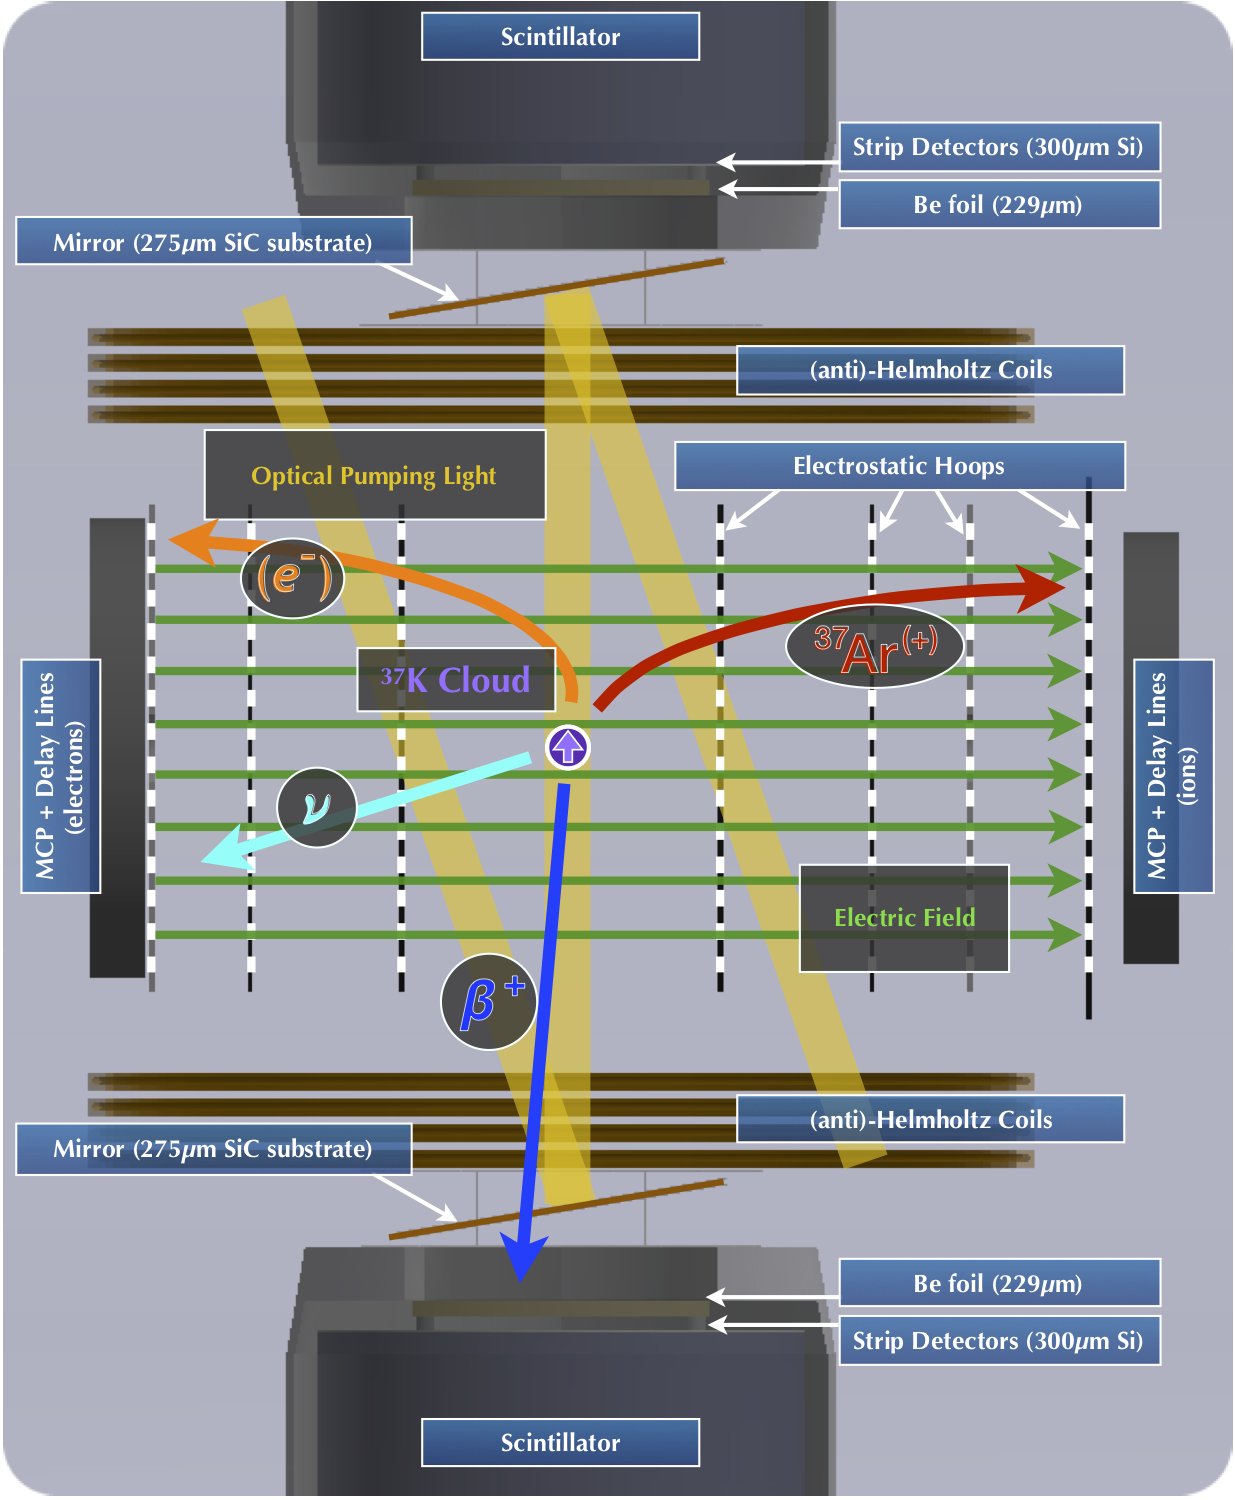
\includegraphics[width=.9\linewidth]{Figures/chamber_cross_section_with_event.png}
	\caption[Diagram of the TRINAT Detection Chamber]{A scale diagram of the interior of the TRINAT detection chamber, shown edge-on with a decay event. After a decay, the daughter will be unaffected by forces from the MOT.  Positively charged recoils and negatively charged shake-off electrons are pulled towards detectors in opposite directions.  Although the $\beta^+$ is charged, it is also highly relativistic and escapes the electric field with minimal perturbation.
	\\
	\\
	% line breaks because somehow it fucks up my equation formatting if I let them go on this same page.  *shrug*
	}
	\note{rMCP is 101.4 mm from center, eMCP is 100 mm from center.  Do I say this somewhere else?}
	\label{chamber_decayevent}
\end{figure}

%%%
\begin{figure}[h!b!t]
	\centering
	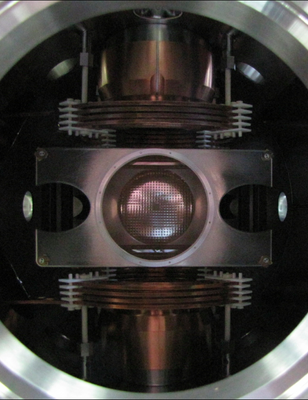
\includegraphics[width=.80\linewidth]{Figures/chamber_photo_2.png}
	\note{Chamber walls are made from 316-L stainless steel, chosen for strength, cost, and minimal eddy currents.}
	\caption[A Photo from Inside the TRINAT Detection Chamber]{Inside the TRINAT detection chamber.  This photo is taken from the vantage point of one of the microchannel plates, looking into the chamber towards the second microchannel plate.  The current-carrying copper Helmholtz coils and two beta telescopes are visible at the top and bottom.  The metallic piece in the foreground is one of the electrostatic hoops used to generate an electric field within the chamber.  The hoop's central circular hole allows access to the microchannel plate, and the two elongated holes on the sides allow the MOT's trapping lasers to pass unimpeded at an angle of 45 degrees `out of the page'.}
	\label{fig:thechamber}
\end{figure}

The detector intended to collect the negatively charged electrons (the ``eMCP'') has an active area of $75.0\,$mm, and is positioned 
%is 75 mm in diameter~\aside{No, it's 86.6 mm in diameter, but the active area is only 75 mm.}and positioned 
$100.0\,$mm from the chamber centre.  It features a Z-stack configuration of three plates, and it is backed by a set of three separate delay lines in a ``hexagonal'' arrangement for redundant position sensitivity (the ``HEX75'').  The detector used to collect positively charged ions (the ``iMCP,'' or equivalently the ``rMCP'' since many of the ions collected are recoils from decay) is $80.0\,$mm in diameter and positioned $101.4\,$mm from the chamber centre.  It features only two plates arranged in a chevron configuration, and it is backed by a set of two separate delay lines (the ``DLD80'') for position sensitivity.  In the context of the present work, the rMCP data is used primarily in conjuction with the photoionization laser to characterize the atom cloud (Section~\ref{photoions}), while the eMCP data is used, together with the beta detectors, as a `tag' for decay events originating from the cloud. \aside{Do I talk about how this works somewhere?  Probably in that section on cuts.}

Due to an unfortunate interaction between the two MCP detectors, during the 2014 beamtime it was not possible to run both the eMCP and the rMCP simultaneously without producing a large background on at least one detector (there seemed to be no consistency as to which detector was most affected at a given time).  As a result, data was instead collected with only one MCP detector biased at a time, and the active detector was alternated every few hours to spend approximately equal time collecting data with the eMCP and rMCP.~\aside{Reference that one table.}  Online scientific data has been collected with the eMCP at electric field strengths of 66.7\,V/cm and 150.\,V/cm, while rMCP data has been collected at 395.\,V/cm, 415.\,V/cm, and 535.\,V/cm.  Note that these field strengths are all too low to significantly perturb any but the least energetic of the (positively charged) betas originating from decay, and those betas already lack the energy that would be needed to travel through the SiC mirror and Be foil vacuum seal into a beta detector. 

The data used to measure the polarization was all collected using the rMCP, while the $\Abeta$ and $\bFierz$ data were collected using the eMCP.  The magnitude of the polarization in each of the two orientations was measured, using online $^{37}$K data, as
\bea
| P_+ | &=& 0.9913 \,\pm\, 0.0008
\\
| P_- | &=& 0.9912 \,\pm\, 0.0009,
\eea
and taken to be the same in both cases --- a result that could only be attained after weeks of optimization using stable $^{41}$K polarization data, with all optical pumping and magnetic field switching parameters kept constant.  The result is described thoroughly within the collaboration's Ref.~\cite{ben_OP}.

%\aside[tag]{JB:  at the level of accuracy you're quoting the answers are in the PRL:  sigma+ P=99.13(8)\%; sigma- -99.12(9)\%}
%an assertion that is backed up by weeks of optimization and polarization data on stable $^{41}$K, with all optical pumping and magnetic field switching parameters kept constant.  

Ambient magnetic field changes of $\sim$50 milliGauss could cause some polarization perturbations at the precision achieved, but the stray fields were kept under control at that level.  The TRINAT lab is in a basement, well shielded from the experimental hall by concrete with rebar, and though 50 mG fields are seen in that hall from an open Helmholtz ion trap, they and the nearby 5-ton crane produce negligible fields when measured at the atom trap. The cyclotron field is $\sim$0.5 Gauss, predominantly vertical, 
but TRINAT's Helmholtz trim coils are adjusted during calibrations with cyclotron both on and off --- and of course the cyclotron is on with a constant field during the $^{37}$K delivery.  Furthermore, because we switched every few hours between the using the eMCP and rMCP, we were able to rule out the possibility that the polarization might have drifted but escaped notice.  

\note[jm]{Here's where Juliette thinks I should've described the polarization methodology better.  ``On page 39 there is a mention of polarization results with no description of the method''}

\section{Beta Detectors}
\label{section:betadetectors}
The beta detectors, located above and below the atom cloud along the axis of polarization (Fig.~\ref{chamber_decayevent}), are each the combination of a plastic scintillator and a set of silicon strip detectors.  Using all of the available information, these detectors are able to reconstruct the energy of an incident beta, as well as its hit position, and provide a timestamp for the hit's arrival.  Together the upper and lower beta detectors subtend approximately 1.4\% of the total solid angle as measured with respect to the cloud position. 

	The two sets of beta detectors were positioned directly along the axis of polarization.  Each beta detector consists of a plastic scintillator and photo-multiplier tube (PMT) \aside{There's gotta be a better way to describe it} placed directly behind a 40$\times$40-pixel double-sided silicon strip detector (DSSD).  \aside{what's the open area of the detector?  how big is each pixel?}  The scintillator is used to measure the overall energy of the incoming particles, as well as to assign a timestamp to these events, while the DSSD is used both to localize the hit position to one (or in some cases, two) individual pixel(s), and also to discriminate between different types of incoming particles.  In particular, though the scintillator will measure the energy of an incoming beta or an incoming gamma with similar efficiency, the beta will lose a portion of its kinetic energy as it passes through the DSSD into the scintillator.  By contrast, an incident gamma will deposit only a very small amount of energy in the DSSD layer, making it possible to reject events with insufficient energy deposited in the DSSD as likely gamma ray events.  Given that the decay of interest to us emits positrons, we expect a persistent background 511 keV gamma rays that are not of interest to us, so it is extremely important that we are able to clean these background events from our spectrum. 


It must be noted that the path between the cloud of trapped atoms and either beta detector is blocked by two objects:  a 275$\,\mu$m silicon carbide mirror (necessary for both trapping and optical pumping), and a 229$\,\mu$m beryllium foil (separating the UHV vacuum within the chamber from the outside world).  In order to minimize beta scattering and energy attenuation, these objects have had their materials selected to use the lightest nuclei with the desired material properties, and have been manufactured to be as thin as possible without compromising the experiment.  As the $^{37}\textrm{K} \rightarrow \,^{37}\textrm{\!Ar} + \beta^{+} + \nu_e$ decay process releases $Q=5.125$\,MeV of kinetic energy~\cite{Q_value}, the great majority of betas are energetic enough to punch through both obstacles without significant energy loss before being collected by the beta detectors.  




%%%% --- * --- %%%%	
\section{The Photoionization Laser}
\label{cloud}
\label{photoions}
In order to measure properties of the trapped $^{37}\textrm{K}$ cloud, a 10\,kHz pulsed laser at 355\,nm is directed towards the cloud.  These photons have sufficient energy to photoionize neutral $^{37}\textrm{K}$ from its excited atomic state, which is populated by the trapping laser when the MOT is active, releasing 0.77\,eV of kinetic energy, but do not interact with ground state $^{37}\textrm{K}$ atoms.  The laser is of sufficiently low intensity that only $\sim 1\%$ of excited state atoms are photoionized, so the technique is only very minimally destructive.
\note{Probably worth mentioning that we test this stuff offline on stable \isotope[41]{K}. But also, surely it should be mentioned in like the AC-MOT/Polarization section too.}

Because an electric field has been applied within this region (Section~\ref{section:field})
the $^{37}\textrm{K}^+$ ions are immediately pulled into the detector on one side of the chamber, while the freed $e^-$ is pulled towards the detector on the opposite side of the chamber.  Because  $^{37}\textrm{K}^+$ is quite heavy relative to its initial energy, it can be treated as moving in a straight line directly to the detector, where its hit position on the microchannel plate is taken as a 2D projection of its position within the cloud.  Similarly, given a sufficient understanding of the electric field, the time difference between the laser pulse and the microchannel plate hit allows for a calculation of the ion's initial position along the third axis.  

\note{As a check:  the camera measurements for photons from de-excitation.  It's aimed 35 degrees from vertical, with its horizontal axis the same as ..... one of the other axes.  I think it's the TOF axis.  I can check this when my computer comes back.   Also, there's an unknown additional delay between some of our DAQ channels that can't be explained by accounting for cable lengths, so we really like having the check there.}
\note[jb1]{JB says:  ``yes, camera x-axis is tof axis.''}


With this procedure, it is possible to produce a precise map of the cloud's position and size, both of which are necessary for the precision measurements of angular correlation parameters that are of interest to us here.  However, it also allows us to extract a third measurement:  the cloud's polarization.

The key to the polarization measurement is that only atoms in the excited atomic state can be photoionized via the 355 nm laser.  While the MOT runs, atoms are constantly being pushed around and excited by the trapping lasers, so this period of time provides a lot of information for characterizing the trap size and position.  When the MOT is shut off, the atoms quickly return to their ground states and are no longer photoionized until the optical pumping laser is turned on.  As described in Section~\ref{sec:op}, and in greater detail in~\cite{ben_OP}, the optical pumping process involves repeatedly exciting atoms from their ground states until the atoms finally cannot absorb any further angular momentum and remain in their fully-polarized (ground) state until they are perturbed.  Therefore, there is a sharp spike in excited-state atoms (and therefore photoions) when the optical pumping begins, and none if 
%\aside[jb1]{JB points out that this should be ``if", not ``once".} 
the cloud has been fully polarized.  The number of photoion events that occur once the sample has been maximally polarized, in comparison with the size and shape of the initial spike of photoions, provides a very precise characterization of the cloud's final polarization~\cite{ben_OP}.


\section{Considerations for Data Collection}
\label{sec:dataconsiderations}
\note[note]{Talk about the data collection.  What types of events are stored?}
There are too many events and the daq is overwhelmed if you record all the events where the eMCP or rMCP is hit.  Although possibly we recorded some with all the eMCP events?  Not sure.
Instead, we record all the events where a scintillator is hit, and all(?) the events where a photoionization laser pulse happens.  It goes at like 10 kHz.  Or maybe it was all the events with a photoionization laser pulse in coincidence with a photoelectron (TOF window) or photoion (TOF window).  But I don't think that's quite right.  That's not what the spectra looked like in the end, so I think that was maybe only for the online plots or something?  Not for the triggers.  Did we clean the non-SOE events in the data acquisition *right then*?  You could do that ok with the electrons, but not so much with the ions.  
\note[tag]{}

